\documentclass[paper=a4, fontsize=11pt]{scrartcl}
\usepackage[T1]{fontenc}
\usepackage[utf8]{inputenc}
\usepackage{lmodern}
\usepackage{multirow}
\usepackage[table,xcdraw]{xcolor}
\usepackage[spanish]{babel}
\usepackage{cite}
\usepackage{amsmath,amsfonts,amsthm} % Math packages
\usepackage{graphics,graphicx, float} %para incluir imágenes y colocarlas
\usepackage[backref,colorlinks=true,linkcolor=black,urlcolor=blue,citecolor=blue]{hyperref} %Para crear enlaces en el pdf
\usepackage{url}
\usepackage[shortlabels]{enumitem}
\usepackage{appendix}
\usepackage{eurosym}
\usepackage{epsfig}
\usepackage{caption}
\usepackage{subcaption}

\usepackage{xcolor}
\usepackage{framed}
\definecolor{shadecolor}{RGB}{239, 251, 255}

\usepackage{listings}
\usepackage{color}

\definecolor{dkgreen}{rgb}{0,0.6,0}
\definecolor{gray}{rgb}{0.5,0.5,0.5}
\definecolor{mauve}{rgb}{0.58,0,0.82}
\definecolor{lgrey}{rgb}{0.9,0.9,0.9}


\lstset{frame=tb,
  language=C++,
  aboveskip=3mm,
  belowskip=3mm,
  showstringspaces=false,
  columns=flexible,
  basicstyle={\small\ttfamily},
  numbers=none,
  numberstyle=\tiny\color{gray},
  keywordstyle=\color{blue},
  commentstyle=\color{dkgreen},
  stringstyle=\color{mauve},
  breaklines=true,
  breakatwhitespace=true,
  tabsize=3
}

\renewcommand{\appendixname}{Anexo}
\renewcommand{\appendixtocname}{Anexo}
\renewcommand{\appendixpagename}{Anexo}

\numberwithin{figure}{section} % Number figures within sections (i.e. 1.1, 1.2, 2.1, 2.2 instead of 1, 2, 3, 4)
\numberwithin{table}{section} % Number tables within sections (i.e. 1.1, 1.2, 2.1, 2.2 instead of 1, 2, 3, 4)
\newcommand{\horrule}[1]{\rule{\linewidth}{#1}} % Create horizontal rule command with 1 argument of height

\title{
    \normalfont \normalsize
    \textsc{{\textbf{Algorítmica (2016-2017)}} \\ Grado en Ingeniería Informática \\ Universidad de Granada} \\ [25pt] % Your university, school and/or department name(s)
    \horrule{0.5pt} \\[0.4cm] % Thin top horizontal rule
    \huge Memoria Práctica 4: Backtracking y Branch & Bound\\ % The assignment title
    \horrule{2pt} \\[0.5cm] % Thick bottom horizontal rule
}
\author{Antonio de la Vega Jiménez }

%*************************************************************


\begin{document}

\maketitle % Muestra el Título
\newpage %inserta un salto de página
\tableofcontents % para generar el índice de contenidos
\listoffigures
\newpage

%*************************************************************

\section{Información PC usado}

\subsection{Hardware}
El hardware usado tiene las siguientes características:
\begin{itemize}
  \item \textbf{CPU:} \texttt{Intel(R) Core(TM) i3 CPU  540}
  \item \textbf{Velocidad reloj:} \texttt{3.07GHz}
  \item \textbf{Caché:} \texttt{4096 KB}
  \item \textbf{RAM:} \texttt{6040128 kB  }
\end{itemize}
\subsection{Software}
\subsubsection{Sistema operativo}
\begin{itemize}
  \item \textbf{SO:} \texttt{Manjaro Linux}
  \item \textbf{Kernel:}\texttt{ 4.4.52-1-MANJARO}
\end{itemize}
\subsubsection{Compilador}
\begin{itemize}
  \item \textbf{Versión compilador:} \texttt{g++ (GCC) 6.3.1 20170306}
\end{itemize}

\section{Algoritmos básicos}

\subsection{Máximo y mínimo}
El código usado es el mostrado a continuación

\begin{lstlisting}
//Obtiene el maximo y el minimo de un vector O(n)
pair<int,int> max_min(const vector<int> &v){

    //Caso base -> El vector tiene solo un elemento
    if(v.size() == 1){
        return pair<int,int> (v[0],v[0]);
    } else {

        //Dividimos en dos mitades
        vector<int> v1(v.begin(), v.begin() + v.size()/2),
               v2(v.begin() + v.size()/2, v.end());
        
        //Llamadas recursivas 
        pair<int,int> m1 = max_min(v1);
        pair<int,int> m2 = max_min(v2);

        pair<int,int> result;
        //Recomponemos la solucion
        result.first = (m1.first > m2.first) ? result.first = m1.first : result.first = m2.first;
        result.second = (m1.second < m2.second) ? result.second = m1.second : result.second = m2.second;

        return result;
    }
}
\end{lstlisting}

\subsubsection{Eficiencia teórica}

 Para obtener la eficiencia observamos las llamadas recursivas:

 Obtenemos la siguiente ecuación de recurrencia:
  \begin{equation}
      T(n) = 2T(n/2) + O(n)
  \end{equation}
  Haciendo uso del método maestro, obtenemos lo siguiente:
  \begin{equation}
      T(n) = O(n^{log_2{2}}) == O(n)
  \end{equation}
  
  Por lo tanto la eficiencia es
  \begin{equation} O(n) \end{equation}.
  


\subsubsection{Eficiencia empírica}

Al representar los datos obtenemos las siguientes gráfica:

\begin{figure}[H]
    \begin{center}
        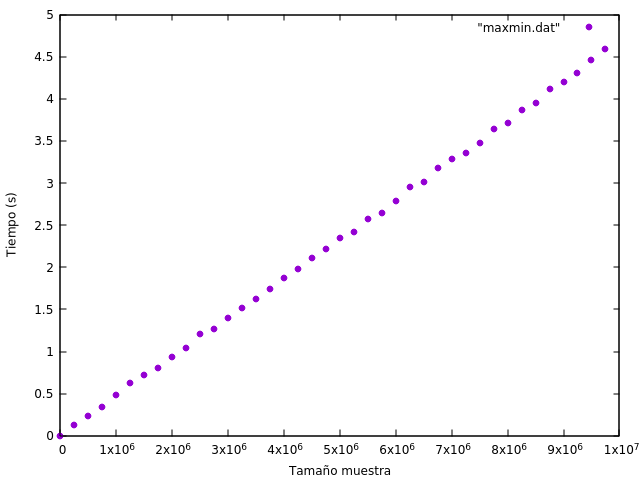
\includegraphics[scale=0.7]{imagenes/g_mm.png}
        \caption{Tiempos de ejecución.}
        \label{fig2}
    \end{center}
\end{figure}

\subsubsection{Ajuste curva teórica a empírica}

En este paso realizamos el siguiente ajuste:
\begin{shaded*}
\begin{verbatim}
gnuplot> f(x)=a*x+b
gnuplot> fit f(x) "maxmin.dat" via a,b

\end{verbatim}
\end{shaded*}

De forma que obtenemos los siguiente parámetros:

\begin{shaded*}
\begin{verbatim}
Final set of parameters            Asymptotic Standard Error
=======================            ==========================
a               = 4.66888e-07      +/- 1.15e-09     (0.2464%)
b               = 0.00284902       +/- 0.006518     (228.8%)

\end{verbatim}
\end{shaded*}

Y finalmente obtenemos la siguiente función ajustada:
\begin{figure}[H]
    \begin{center}
        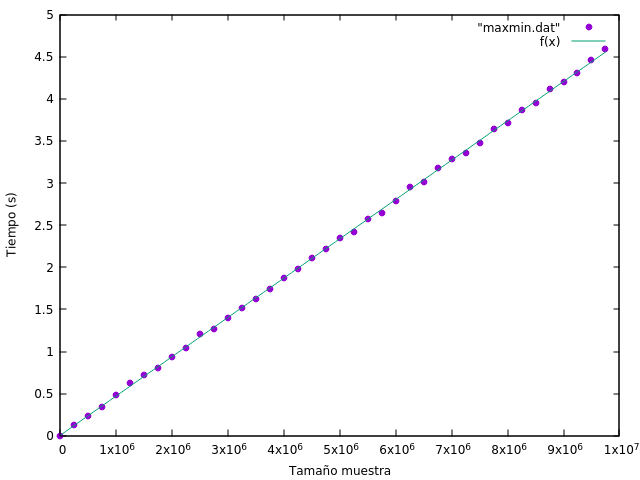
\includegraphics[scale=0.7]{imagenes/mm_adj.png}
        \caption{Ajuste eficiencia teórica y empírica.}
        \label{fig3}
    \end{center}
\end{figure}

%*************************************
%*************************************
%*************************************
%*************************************



\section{Tornillos y tuercas}

El código usado es el mostrado a continuación

\begin{lstlisting}
vector<pair<int,int> > agrupartt(vector<int> &tornillos, vector<int> &tuercas) {

    //Caso base
    if(tornillos.size() <= 1) {
        vector<pair<int,int> > tt;
        if(tornillos.size() == 1) {
            pair<int,int> tornillo_tuerca(tornillos.at(0),tuercas.at(0));
            tt.push_back(tornillo_tuerca);
        }
        return tt;
    } else {

        int tornillo_pivote = tornillos.at((int)tornillos.size()/2);
        vector<int> tuercas_menores,tuercas_mayores,tuerca_igual;

        for(int i: tuercas) {
            if(i < tornillo_pivote) {
                tuercas_menores.push_back(i);
            } else if (i > tornillo_pivote) {
                tuercas_mayores.push_back(i);
            } else {
                tuerca_igual.push_back(i);
            }
        }

        int tuerca_pivote = tuerca_igual.at(0);
        vector<int> tornillos_menores,tornillos_mayores,tornillo_igual;

        for(int i: tornillos) {
            if(i < tuerca_pivote) {
                tornillos_menores.push_back(i);
            } else if (i > tuerca_pivote) {
                tornillos_mayores.push_back(i);
            } else {
                tornillo_igual.push_back(i);
            }
        }

        vector<pair<int,int> > tt1,tt2,tt3;

        //Llamadas recursivas
        tt1 = agrupartt(tornillo_igual,tuerca_igual);
        tt2 = agrupartt(tornillos_mayores,tuercas_mayores);
        tt3 = agrupartt(tornillos_menores,tuercas_menores);

        //Recomponer la solucion
        vector<pair<int,int> > tornillos_tuercas;
        tornillos_tuercas.insert(tornillos_tuercas.end(),tt1.begin(),tt1.end());
        tornillos_tuercas.insert(tornillos_tuercas.end(),tt2.begin(),tt2.end());
        tornillos_tuercas.insert(tornillos_tuercas.end(),tt3.begin(),tt3.end());

        return tornillos_tuercas;
    }
}
\end{lstlisting}


\subsubsection{Eficiencia teórica}

Para obtener la eficiencia observamos las llamadas recursivas:

 Obtenemos la siguiente ecuación de recurrencia:
  \begin{equation}
      T(n) = 3T(n/3) + O(1)
  \end{equation}
  Haciendo uso del método maestro, como el segundo tiempo es constante, obtenemos lo siguiente:
  \begin{equation}
      T(n) = O(n^{log_3{3}})
  \end{equation}
  
  Por lo tanto la eficiencia es
  \begin{equation} O(n) \end{equation}.
  


\subsubsection{Eficiencia empírica}

Al representar los datos obtenemos las siguientes gráfica:

\begin{figure}[H]
    \begin{center}
        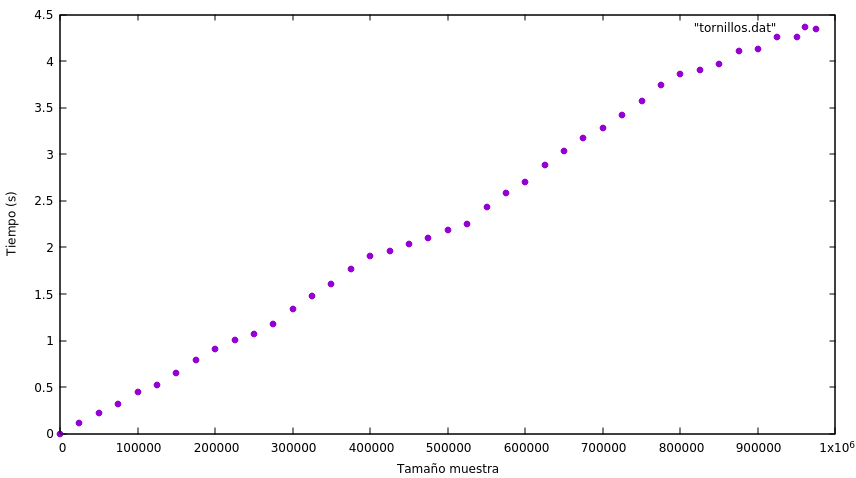
\includegraphics[scale=0.7]{imagenes/g_tt.png}
        \caption{Tiempos de ejecución.}
        \label{fig19}
    \end{center}
\end{figure}

\subsubsection{Ajuste curva teórica a empírica}

\begin{shaded*}
\begin{verbatim}
gnuplot> f(x) = a*x + b
gnuplot> fit f(x) "tornillos.dat" via a,b

\end{verbatim}
\end{shaded*}

De forma que obtenemos los siguiente parámetros:

\begin{shaded*}
\begin{verbatim}
Final set of parameters            Asymptotic Standard Error
=======================            ==========================
a               = 4.67228e-06      +/- 4.206e-08    (0.9002%)
b               = -0.0387318       +/- 0.02383      (61.52%)

\end{verbatim}
\end{shaded*}

Y finalmente obtenemos la siguiente función ajustada:
\begin{figure}[H]
    \begin{center}
        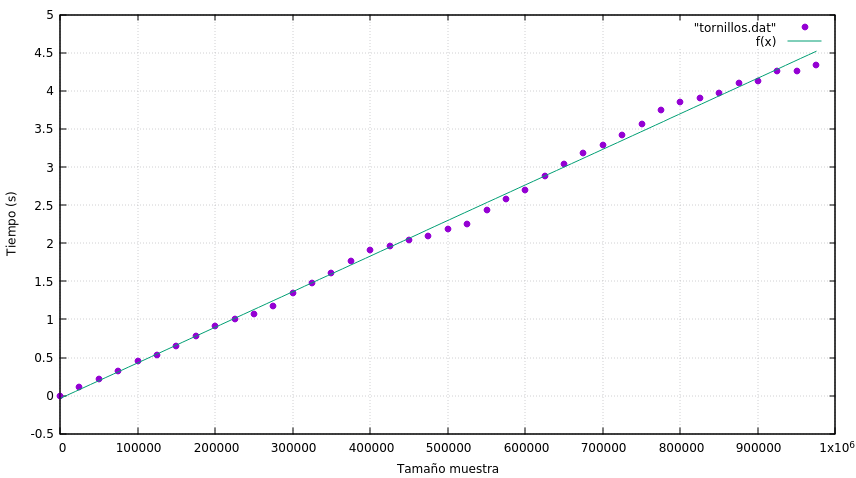
\includegraphics[scale=0.7]{imagenes/tt_adj.png}
        \caption{Ajuste eficiencia teórica y empírica.}
        \label{fig20}
    \end{center}
\end{figure}


%*************************************
%*************************************
%*************************************
%*************************************
\section{Alicatado suelo}
\begin{figure}[H]
    \begin{center}
        
\includegraphics[scale=0.5]{imagenes/test.png}
        \caption{Ejemplo salida.}
        \label{fig2}
    \end{center}
\end{figure}

El código usado es el mostrado a continuación

\begin{lstlisting}
void alicatar(vector<vector<int> > &suelo, pair<int,int> desague, pair<int,int> esq, int lado=-1) {
    static int count = 0;
    int x,y;
    x = esq.first;
    y = esq.second;

    count++;

    if(lado == -1) {
        x = 0;
        y = 0;
        lado = suelo.at(0).size();
        suelo[desague.first][desague.second] = -1 ;
    }

    //CASO BASE
    if(lado == 2) {
        for(int i=0; i < 2; i++)
            for(int j=0; j <2 ; j++ )
                if(suelo.at(i+x).at(j+y) == 0)
                    suelo.at(i+x).at(j+y) = count;

        return;

        //LLAMADAS RECURSIVAS
    } else {

        int cua = cuadrante(x,y,lado,desague);
        int nlado = lado/2;

        pair<int,int> esq1(x, y);
        pair<int,int> des1(x+nlado-1,y+nlado-1);

        pair<int,int> esq2(x, y+nlado);
        pair<int,int> des2(x+nlado-1,y+nlado);

        pair<int,int> esq3(x+nlado, y);
        pair<int,int> des3(x+nlado,y+nlado-1);

        pair<int,int> esq4(x+nlado, y+nlado);
        pair<int,int> des4(x+nlado, y+nlado);

        if(cua == 1) {
            suelo.at(des2.first).at(des2.second) = count;
            suelo.at(des3.first).at(des3.second) = count;
            suelo.at(des4.first).at(des4.second) = count;

            alicatar(suelo,desague,esq1,nlado);
            alicatar(suelo,des2,esq2,nlado);
            alicatar(suelo,des3,esq3,nlado);
            alicatar(suelo,des4,esq4,nlado);

        } else if (cua == 2) {
            suelo.at(des1.first).at(des1.second) = count;
            suelo.at(des3.first).at(des3.second) = count;
            suelo.at(des4.first).at(des4.second) = count;

            alicatar(suelo,des1,esq1,nlado);
            alicatar(suelo,desague,esq2,nlado);
            alicatar(suelo,des3,esq3,nlado);
            alicatar(suelo,des4,esq4,nlado);

        } else if (cua == 3) {
            suelo.at(des1.first).at(des1.second) = count;
            suelo.at(des2.first).at(des2.second) = count;
            suelo.at(des4.first).at(des4.second) = count;

            alicatar(suelo,des1,esq1,nlado);
            alicatar(suelo,des2,esq2,nlado);
            alicatar(suelo,desague,esq3,nlado);
            alicatar(suelo,des4,esq4,nlado);
        } else {
            suelo.at(des1.first).at(des1.second) = count;
            suelo.at(des2.first).at(des2.second) = count;
            suelo.at(des3.first).at(des3.second) = count;

            alicatar(suelo,des1,esq1,nlado);
            alicatar(suelo,des2,esq2,nlado);
            alicatar(suelo,des3,esq3,nlado);
            alicatar(suelo,desague,esq4,nlado);
        }

        return;
    }
}}    
}
\end{lstlisting}


\subsubsection{Eficiencia teórica}

Para obtener la eficiencia observamos las llamadas recursivas:

 Obtenemos la siguiente ecuación de recurrencia:
  \begin{equation}
      T(n) = 4T(n/2) + O(1)
  \end{equation}
  Haciendo uso del método maestro, como el segundo tiempo es constante, obtenemos lo siguiente:
  \begin{equation}
      T(n) = O(n^{log_2{4}})
  \end{equation}
  
  Por lo tanto la eficiencia es
  \begin{equation} O(n^2 ) \end{equation}.
  

\subsubsection{Eficiencia empírica}

Al representar los datos obtenemos las siguientes gráfica:

\begin{figure}[H]
    \begin{center}
        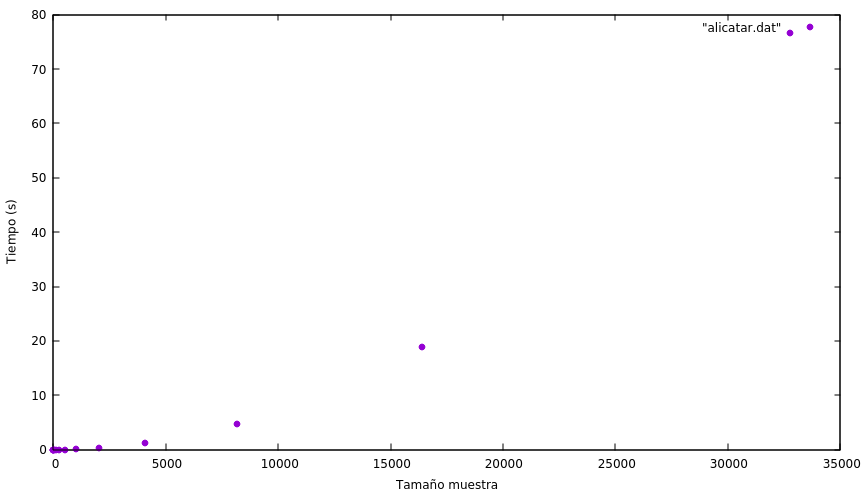
\includegraphics[scale=0.7]{imagenes/g_a.png}
        \caption{Tiempos de ejecución.}
        \label{fig11}
    \end{center}
\end{figure}


\subsubsection{Ajuste curva teórica a empírica}

En este paso realizamos el siguiente ajuste:
\begin{shaded*}
\begin{verbatim}
gnuplot> f(x) = a*x*x + b*x + c
gnuplot> fit f(x) "alicatar.dat" via a,b,c

\end{verbatim}
\end{shaded*}

De forma que obtenemos los siguiente parámetros:

\begin{shaded*}
\begin{verbatim}
Final set of parameters            Asymptotic Standard Error
=======================            ==========================
a               = 7.2163e-08       +/- 1.521e-10    (0.2107%)
b               = -2.58945e-05     +/- 4.697e-06    (18.14%)
c               = 0.0142352        +/- 0.01391      (97.7%)

\end{verbatim}
\end{shaded*}

Y finalmente obtenemos la siguiente función ajustada:
\begin{figure}[H]
    \begin{center}
        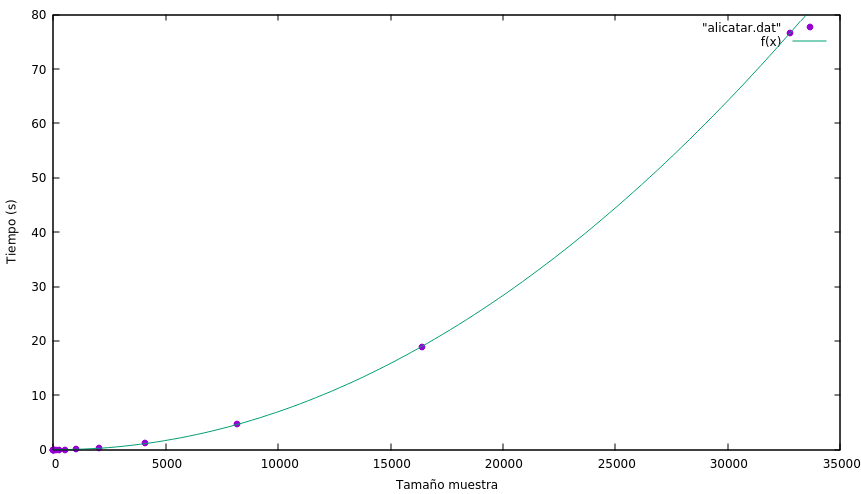
\includegraphics[scale=0.7]{imagenes/a_adj.png}
        \caption{Ajuste eficiencia teórica y empírica.}
        \label{fig13}
    \end{center}
\end{figure}


%*************************************************************
\newpage

\end{document}
